%Input preamble
\documentclass[11pt]{article}

% colors
\usepackage[table]{xcolor}
\definecolor{maroon}{RGB}{153,0,18}
\definecolor{lime}{RGB}{190,213,88}
\definecolor{sand}{RGB}{217,202,179}
\definecolor{fire}{RGB}{144,50,61}
\definecolor{brick}{RGB}{94,11,21}
\definecolor{olive}{RGB}{117,109,84}
\definecolor{lavpink}{RGB}{172,123,132}
\definecolor{darkpurp}{RGB}{49,10,49}
\definecolor{salmon}{RGB}{204,90,113}
\definecolor{mauve}{RGB}{94,73,85}
\definecolor{greyblue}{RGB}{125,132,145}
\definecolor{greypurp}{RGB}{68,56,80}
\definecolor{brightpurp}{RGB}{96,20,255}

% packages (please add in alphabetical order)
\usepackage{adjustbox}
\usepackage{amsfonts}
\usepackage{amsmath}
\usepackage{amssymb}
\usepackage{array}
\usepackage{bm}
\usepackage{booktabs}
\usepackage{caption}
\usepackage{epstopdf}
\usepackage{float}
\usepackage[margin=1in]{geometry}
\usepackage{graphicx}
\usepackage[colorlinks=true, linkcolor=brightpurp, citecolor=brightpurp, urlcolor=salmon]{hyperref}
\usepackage{lipsum}
\usepackage{longtable}
\usepackage{mathtools}
\usepackage{multirow}
\usepackage{natbib}
\usepackage{rotating}
\usepackage{setspace}
\usepackage{subcaption}
%\usepackage{threeparttable}
\usepackage{threeparttablex}
\usepackage{xr}
\usepackage[printwatermark]{xwatermark}


\newcolumntype{L}[1]{>{\raggedright\let\newline\\\arraybackslash\hspace{0pt}}m{#1}}
\newcolumntype{C}[1]{>{\centering\let\newline\\\arraybackslash\hspace{0pt}}m{#1}}
\newcolumntype{R}[1]{>{\raggedleft\let\newline\\\arraybackslash\hspace{0pt}}m{#1}}

% commands
\newcommand{\mr}{\multirow}
\newcommand{\mc}{\multicolumn}

%Other parameters
\newcommand{\noutcomes}{95}
\newcommand{\treatsubsabc}{$75\%$}
\newcommand{\treatsubscarec}{$74\%$}
\newcommand{\treatsubscaref}{$63\%$}

%Counts
%Males
\newcommand{\positivem}{$79\%$}
\newcommand{\positivesm}{$37\%$}

%Females
\newcommand{\positivef}{$73\%$}
\newcommand{\positivesf}{$35\%$}

%Counts, control substitution
%Males
\newcommand{\positivecsnm}{$58\%$}
\newcommand{\positivescsnm}{$25\%$}

\newcommand{\positivecsam}{$74\%$}
\newcommand{\positivescsam}{$38\%$}

%Females
%% no alternative
\newcommand{\positivecsnf}{$83\%$}
\newcommand{\positivescsnf}{$46\%$}

%% alternative
\newcommand{\positivecsaf}{$73\%$}
\newcommand{\positivescsaf}{$23\%$}

%Pooled

%Effects
%Males

%Females
\newcommand{\hsgradf}{$7$}
\newcommand{\yearsedf}{$1.2$}



%Pooled

%CBA
%IRR
%Males
\newcommand{\irrm}{$15\%$}
\newcommand{\irrsem}{$13\%$}

%Females
\newcommand{\irrf}{$10\%$}
\newcommand{\irrsef}{$12\%$}

%Pooled
\newcommand{\irrp}{$13\%$}
\newcommand{\irrsep}{$11\%$}

%BC
%Males
\newcommand{\bcm}{$7.88$}
\newcommand{\bcsem}{$8.06$}

%Females
\newcommand{\bcf}{$2.30$}
\newcommand{\bcsef}{$1.56$}

%Pooled
\newcommand{\bcp}{$4.35$}
\newcommand{\bcsep}{$2.57$}

%NPV streams
%Pooled
\newcommand{\parincomenpvp}{$\$115,026$}

\externaldocument{abc_comprehensivecba}
\externaldocument{abc_comprehensivecba}
\externaldocument{abc_comprehensivecba}
\pagenumbering{roman}

\begin{document}

\begin{titlepage}

\title{\Large \textbf{HOLDING TANK \\  Quantifying the Life-cycle Benefits of a Prototypical Early Childhood Program}}

\date{This Draft: \today}

\maketitle

\end{titlepage}

\clearpage

\doublespacing

\setcounter{page}{0}
\pagenumbering{arabic}\

\subsection{Randomization Protocol and Compromises} \label{section:randomization}

Randomization for ABC/CARE was conducted on child pairs matched on family background. Siblings and twins were jointly randomized into either treatment or control groups.\footnote{For siblings, this occurred when two siblings were close enough in age such that both of them were eligible for the program.} Randomization pairing was based on a risk index, maternal education, maternal age, and gender of the subject.\footnote{We do not know the original pairs.} ABC collected an initial sample of 121 subjects. We characterize each missing observation in Appendix~\ref{appendix:background}. In Appendix~\ref{appendix:estimates}, we document that our estimates are robust when we adjust for missing data using standard methods, described in Appendix~\ref{app:method_partialobs}. We conduct the same analysis for the CARE sample. 22 subjects in ABC did not stay in the program through age 5. Dropouts are evenly balanced and are primarily related to the health of the child and mobility of families and not to dissatisfaction with the program.\footnote{The 22 dropouts include four children who died, four children who left the study because their parents moved, and two children who were diagnosed as developmentally delayed. Details are in Table~\ref{table:abccompromises}. Everyone offered the program was randomized to either treatment or control. All eligible families agreed to participate. Dropping out occurs \emph{after} randomization.}

\subsection{Control Group Substitution}

In ABC/CARE, many control group members (but no children from families offered treatment) attended alternative (to home) childcare or preschool centers.\footnote{See \cite{Heckman_Hohmann_etal_2000_QJE} on the issue of substitution bias in social experiments.} The figure is \treatsubsabc\ for ABC and \treatsubscarec\ for CARE.

\begin{sidewaysfigure}[!htbp]
\centering
\caption{Control Substitution Characteristics, ABC/CARE Control Group}\label{fig:control-sub}
\begin{subfigure}[h]{0.49\textwidth}
	\centering
	\caption{Cumulative Enrollment} \label{fig:treatsubcare}
	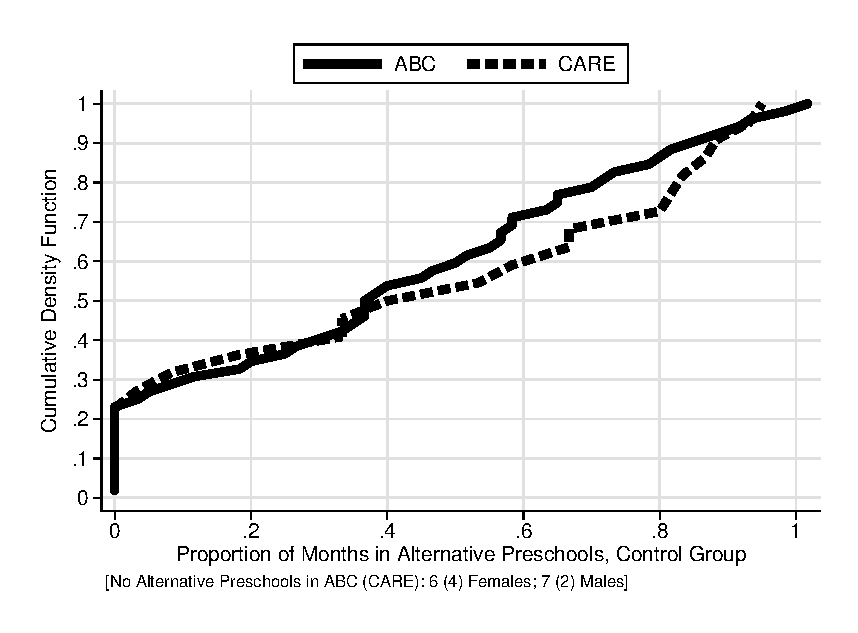
\includegraphics[width=\textwidth]{output/abccare_controlcontamination.eps}
\end{subfigure}
\begin{subfigure}[h]{0.49\textwidth}
	\centering
	\caption{Enrollment Dynamics} \label{fig:proportion-alt-pre}
	\includegraphics[width=\textwidth]{output/abccare_Vprobs.eps}
\end{subfigure}%
\footnotesize \justify
Note: Panel (a) displays the cumulative distribution function of enrollment in alternatives. Panel (b) displays the fraction of ABC/CARE control-group children enrolled in alternatives, conditional on being enrolled in the previous age (at least one month).\\
\end{sidewaysfigure}

Figure~\ref{fig:treatsubcare} shows the cumulative distribution of the proportion of time in the first five years that control subjects were enrolled in alternatives. Figure~\ref{fig:proportion-alt-pre} shows the dynamics of enrollment. Those who enroll generally stay enrolled. As control children age, they are more likely to enter childcare (see Appendix~\ref{app:control-subbb}).

Children in the control group who are enrolled in alternative early childcare programs are less economically disadvantaged at baseline compared to children who stay at home. Disadvantage is measured by maternal education, maternal IQ, Apgar scores, and the high-risk index defining ABC/CARE eligibility. Children who attend alternatives have fewer siblings. On average, they are children of mothers who are more likely to be working at baseline.\footnote{Statistically significant at 10\%.} Parents of girls are much more likely to use alternative childcare if assigned to the control group.\footnote{See Table~\ref{table:controlsubscharacteristics} in Appendix~\ref{appendix:background} for tests of differences across these variables between children in the control group who attended and who did not attend alternative preschools.}

Most of the alternative childcare centers received federal subsidies and were subject to the federal regulations of the era.\footnote{Appendix~\ref{appendix:tetanus} discusses the federal standards of that day. See \citet{Department-of-Health_1968_DayCareRequirements,NCGA_1971_House-Bill-100,Ramey-et-al_1977_Intro-to-ABC,Ramey_Campbell_1979_SR,Ramey_McGinness_etal_1982_Abecedarianapproach, Burchinal_Campbell_etal_1997_CD}.} They had relatively low quality compared to ABC/CARE.\footnote{When we compare ABC/CARE treatment to these alternatives, ABC/CARE has substantial treatment effects. Further, as we argue below, parents perceived that ABC/CARE was superior to the alternatives.} The access of control-group children to alternative programs affects the interpretation of estimated treatment effects, as we discuss next.

\section{Summarizing Multiple Treatment Effects} \label{section:methodology}

ABC/CARE has rich longitudinal data on multiple outcomes over multiple periods of the life cycle. Summarizing these effects in an interpretable way is challenging.\footnote{Appendix~\ref{appendix:results} presents step-down $p$-values for the blocks of outcomes that are used in our benefit/cost analysis which we summarize in this section (\citealp{Lehman_Romano_2005_AnnStat} and \citealp{Romano_Shaikh_2006_AnnStat}). We follow the algorithm in \citet{Romano_Wolf_2016_pval_SaPL}.} Simpler, more digestible summary measures are useful for understanding our main findings. This section discusses our approach to summarizing vectors of treatment effects using combining functions that count the proportion of treatment effects by different categories of outcomes.

Consider a block of $N_l$ outcomes indexed by set $Q_l = \{1,\dots,N_l\}$. Let $j \in Q_l$ be a particular outcome within block $l$. Associated with it is a mean treatment effect
\begin{equation}
\Delta_{j,a} : = \mathbb{E} \left[ Y^1_{j,a} - Y^0_{j,a} | \bm{B} \in \mathcal{B}_0 \right], j \in Q_l.
\end{equation}

We assume that outcomes can be ordered so that $\Delta_{j,t} >0$ is beneficial.\footnote{All but 5\% of the outcomes we study can be ranked in this fashion. See Appendix~\ref{appendix:results} for a discussion.} We summarize the estimated effects of the program on outcomes within the block by the count of positive impacts within block $l$:
\begin{equation}
C_l = \sum^{N_l}_{j=1} 1 (\hat{\Delta}_{j,a} >0).
\end{equation}
The proportion of beneficial outcomes in block $l$ is $C_l / N_l$.\footnote{In our empirical application we consider all the outcomes as a block, and then different blocks grouped according to common categories---e.g., skills, health, crime.}

Let $\mathcal{L}$ be the set of blocks. Under the null hypothesis of no treatment effects for all $j \in Q_l, l \in \mathcal{L}$, and assuming the validity of asymptotic approximations, $C_l / N_l$ should be centered around $1/2$. This is true regardless of any statistical dependence among the outcomes. We bootstrap to obtain $p$-values for the null for each block and over all blocks. Bootstrapping allows us to account for dependence across outcomes in a general way. We also count the beneficial treatment effects that are statistically significant in the sets of outcomes across each of the groups indexed by the set $Q_l$. Using a 10\% significance level, on average 10\% of all outcomes should be ``significant'' at the 10\% level even if there is no treatment effect of the program. We provide evidence against both null hypotheses.\footnote{In this case, we perform a ``double bootstrap'' procedure to first determine significant treatment effects at $10\%$ level and then calculate the standard error of the count.} Combining counts across all blocks enables us to avoid (i) arbitrarily picking outcomes that have statistically significant effects---``cherry picking''; or (ii) arbitrarily selecting blocks of outcomes to correct the $p$-values when accounting for multiple hypothesis testing.\footnote{We present $p$-values for these hypotheses and a number of combining functions by outcome categories in Appendix~\ref{appendix:results}.}$^{\text{,}}$\footnote{In Appendix~\ref{appendix:results} we present yet another alternative. We calculate a ``latent'' outcome out of the set of outcomes within a block and perform inference on this latent. The results point to beneficial effects of the program in this case as well.}

\section{Estimated Treatment Effects and Combining Functions}\label{section:c-functions}

ABC/CARE has a multiplicity of treatment effects corresponding to all of the measures collected in the multiple waves of the longitudinal surveys. Reporting these treatment effects in the text would overwhelm the reader. In Web Appendix~\ref{appendix:results}, we report estimates of the main treatment effects that underlie our benefit/cost and rate of return analyses.\footnote{Web Appendix~\ref{appendix:results} reports treatment effects and step-down $p$-values for all the outcomes analyzed. These account for multiple hypothesis testing as in \citet{Lehman_Romano_2005_AnnStat} and \citet{Romano_Shaikh_2006_AnnStat}.} These treatment effects are monetized in Section~\ref{section:cbamethodology} to present an economically justified aggregate measure.

Evidence from ABC/CARE and many other early childhood programs is often criticized because of their small sample sizes.\footnote{See, e.g., \cite{Murray_2013_GivingKids_JJHBOOK}.} An extensive analysis reported in \citet{Campbell_Conti_etal_2014_EarlyChildhoodInvestments} shows that asymptotic inference and small sample permutation-based inference closely agree when applied to ABC/CARE data. For this reason, we use large sample inference throughout this paper.\footnote{For precise details on the construction of the inference procedures used throughout the paper, see Appendix~\ref{appendix:bootstrap}.}

\subsection{Estimated Combining Functions}

We report estimates of the proportion of beneficial effects by block and overall.\footnote{We consider a total of 95 outcomes that we classify in Appendix~\ref{appendix:results}. \textbf{[JJH: Jorge, fix G and discuss]} These are the outcomes that most clearly relate to the treatment offered by the program.} The analysis is based on treatment effect \eqref{eq:effect}. Figure~\ref{fig:ppositive} displays the results from this analysis: ABC/CARE positively impacted a large percentage of the outcomes. We show the counts for treatment compared to the next best alternative chosen by parents in Figure~\ref{fig:ppositivenb}. Proportionately more outcomes are beneficial for females, but the proportions are high for both groups and well above the benchmark of 1/2. In Tables~\ref{table:abccare_rslt_pooled_counts} to \ref{table:abccare_rslt_female_counts_n10a10} of Appendix~\ref{appendix:results}, we document a large and precisely determined fraction of beneficial treatment effects well above one half for both genders for categories of outcomes spanning the life cycle through the mid 30's.

Using an $\alpha$-level of significance, one would expect to find that $\alpha\%$ of the treatment effects are ``statistically significant,'' even if the null hypothesis of no effect of the program is true simply by chance. At a 10\% level of significance, $46\%$ are statistically significant for females and $28\%$ for males (see Figure~\ref{fig:ppositive10}).

Figures~\ref{fig:ppositivehome} and Figure~\ref{fig:ppositivealternative} adjust the count in Figure~\ref{fig:ppositivenb} to analyze more clearly defined counterfactuals: treatment compared to staying at home and treatment compared to alternative preschool. These comparisons indicate that girls and boys benefit differently from alternatives to high quality treatment. Compared across all categories, girls benefit more from treatment when compared to staying at home (as opposed to attending alternative childcares), while males benefit more from treatment when compared to attending an alternative childcare arrangement (as opposed to staying at home).

\begin{sidewaysfigure}[!htbp]
\centering
\caption{Positively Impacted Outcomes, ABC/CARE Males and Females}\label{fig:ppositive}
\begin{subfigure}[h]{0.4\textwidth}
		\centering
		\caption{Treatment vs. Next Best} \label{fig:ppositivenb}
		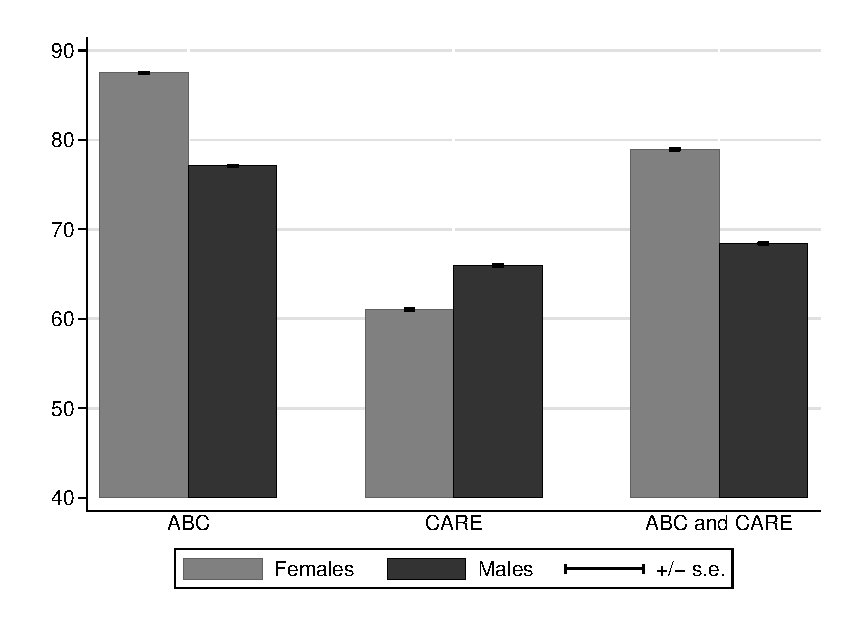
\includegraphics[width=\textwidth]{output/itt_noctrl_all.eps}
\end{subfigure}%
\begin{subfigure}[h]{0.4\textwidth}
	\centering
	\caption{Treatment vs. Next Best, Significant at 10\% Level} \label{fig:ppositive10}
		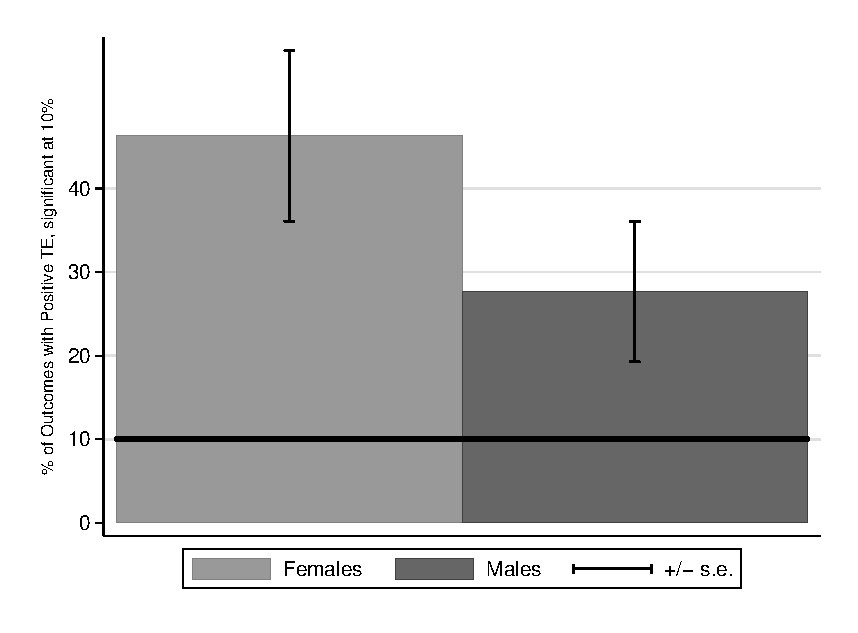
\includegraphics[width=\textwidth]{output/itt_noctrl_all_sig10.eps}
\end{subfigure}
\begin{subfigure}[h]{0.4\textwidth}
		\centering
		\caption{ Treatment vs. Stay at Home} \label{fig:ppositivehome}
		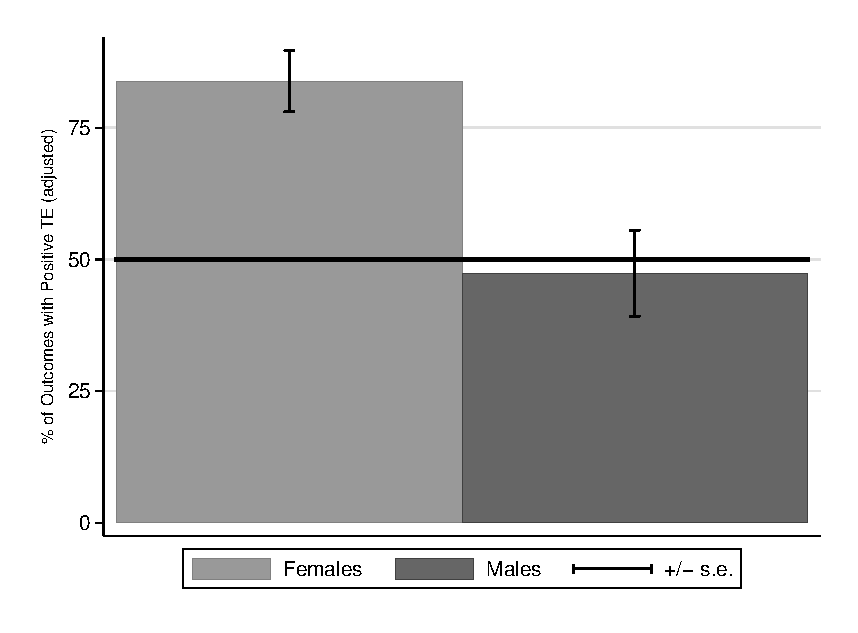
\includegraphics[width=\textwidth]{output/epan_ipw_p0_all.eps}
\end{subfigure}%
\begin{subfigure}[h]{0.4\textwidth}
	\centering
	\caption{Treatment vs. Alternative Preschool} \label{fig:ppositivealternative}
		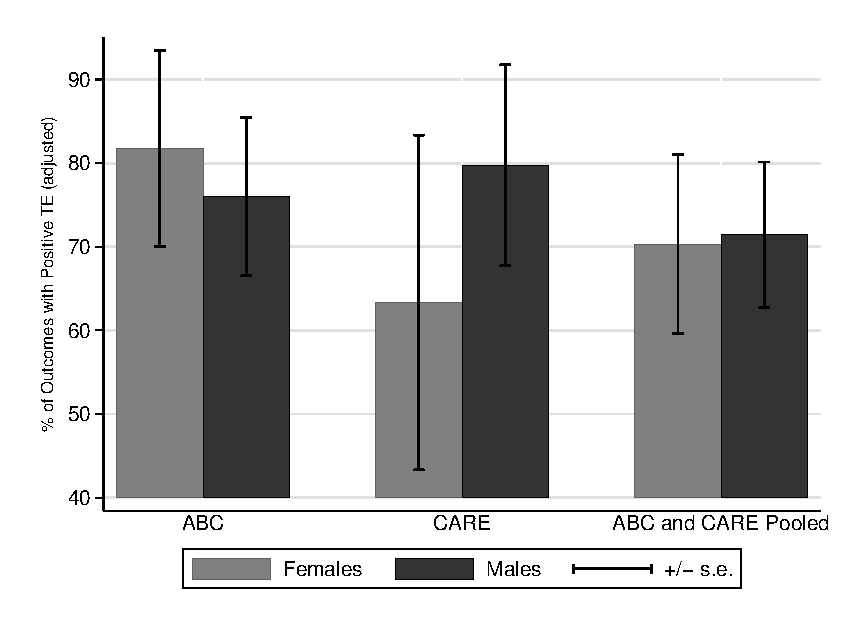
\includegraphics[width=\textwidth]{output/epan_ipw_p1_all.eps}
\end{subfigure}
\scriptsize \justify
Note: Panel (a) percentage of outcomes displaying a positive treatment effect, comparing treatment to next best. Panel (b) percentage of outcomes displaying a positive and statistically significant treatment effect (10\% significance level). Panel (c) displays the percentage of outcomes with a positive treatment effect, comparing treatment to staying at home. Panel (d) displays the percentage of outcomes with a positive treatment effect, comparing treatment to alternative childcare arrangements. Standard errors are based on the empirical bootstrap distribution. For Panel (b) we perform a ``double bootstrap'' procedure to first determine significant treatment effects at $10\%$ level and then calculate the standard error of the count.\\
\end{sidewaysfigure}

\section[Background and Data Sources]{Background and Data Sources} \label{section:background}
\subsection{Overview}

ABC/CARE targeted disadvantaged, predominately African-American children in Chapel Hill/Durham, North Carolina.\footnote{Both ABC and CARE were designed and implemented by researchers at the Frank Porter Graham Center of the University of North Carolina in Chapel Hill.} Table~\ref{tab:programcomparison} compares the two virtually identical programs. Appendix~\ref{appendix:background} describes these programs in detail. Here, we summarize their main features.

The goal of these programs was to enhance the early-life skills of disadvantaged children. Both programs supported language, motor, and cognitive development as well as socio-emotional competencies considered crucial for school success including task-orientation, ability to communicate, independence, and pro-social behavior.\footnote{\citet{Ramey_Collier_etal_1976_CarolinaAbecedarianProject, Ramey_etal_1985_Project-CARE_TiECSE, Sparling_1974_Synth_Edu_Infant_SPEECH, Wasik_Ramey_etal_1990_CD, Ramey-etal_2012-ABC}.}

The programs individualized treatment. Each child's progress was recorded and learning activities were appropriately adjusted every 2 to 3 weeks. Environments were organized to promote pre-literacy and provide access to a rich set of learning tools.\footnote{The ``LearningGames'' approach was implemented by infant and toddler caregivers in 1:1 child-adult interactions. Each ``LearningGames'' activity states a developmentally-appropriate objective, the necessary materials, directions for teacher behavior, and expected child outcome.} The curriculum emphasized active learning experiences, dramatic play, and basic concepts of order and category (``pre-academic skills''), as well as discipline and the ability to interact with and respect others.  At later ages (3 through 5), the program focused on the development of ``socio-linguistic and communicative competence.''\footnote{\citet{Ramey-et-al_1977_Intro-to-ABC, Haskins_1985_CD, Ramey_1981_Modification, Ramey_Campbell_1979_SR, Ramey_Smith_1977_AJMD, Ramey_McGinness_etal_1982_Abecedarianapproach, Sparling_Lewis_1979_BOOKLearninggamesFirstThree,Sparling_Lewis_1984_BOOKLearningGamesThreesFours}.}

ABC recruited four cohorts of children born between 1972 and 1976. CARE recruited two cohorts of children, born between 1978 and 1980. The recruitment processes for each study were identical. Potential participant families were referred to researchers by local social service agencies and hospitals at the beginning of the mother's last trimester of pregnancy. Eligibility was determined by a score on a childhood risk index.\footnote{See Appendix~\ref{appendix:background} for details on the construction for the index used. The index weighs the following variables (listed from the most to the least important according to the index): maternal and paternal education, family income, father's presence at home, lack of maternal relatives in the area, siblings behind appropriate grade in school, family in welfare, father in unstable job, maternal IQ, siblings' IQ, social agency indicates that the family is disadvantaged, one or more family members has sought a form of professional help in the last three years, and any other special circumstance detected by program's staff.}

As shown in Table~\ref{tab:programcomparison}, the design and implementation of ABC and CARE were very similar. ABC had two phases, the first of which lasted from birth until age 5. In this phase, children were randomly assigned to treatment. The second phase of the study consisted of child academic support through home visits from ages 5 through 8. CARE consisted of two treatment phases as well that were very similar to ABC. The first phase of CARE from birth until age 5, had an additional treatment arm of home visits designed to improve home environments.\footnote{\citet{Wasik_Ramey_etal_1990_CD}.} Participation in the second phase was randomized in ABC, but not in CARE.

Our analysis is based on the first phase and pools the CARE treatment group with the ABC treatment group. The second-phase treatment of ABC/CARE had little impact on participants (for evidence, see \citealp{Campbell_Conti_etal_2014_EarlyChildhoodInvestments} and \citealp{ABCCARE_Dataset}). \citet{Campbell_Conti_etal_2014_EarlyChildhoodInvestments} establish the validity of pooling the data on second phase treatments and controls with the first phase controls in ABC.

We do not use the data on the CARE group that only received home visits in the early years. \citet{Campbell_Conti_etal_2014_EarlyChildhoodInvestments} and \citet{ABCCARE_Dataset} show that there is no statistically significant effect of this component.

For the treatment phase that we analyze, the center received the treated children from 7:45 a.m. to 5:30 p.m, five days a week and fifty weeks a year. As we argue below, in practice the center had a very relevant childcare component that caused gains in parental labor income.

\begin{table}[!htbp]
\centering
\caption{ABC and CARE, Program Comparison} \label{tab:programcomparison}
\begin{adjustbox}{max width=\textwidth}
\begin{threeparttable}
	\small
	\begin{table}[H]
\begin{center}
\begin{threeparttable}
\caption{ABC and CARE, Programs Comparison} \label{tab:programcomparison}
\scriptsize
\scalebox{.9}{\begin{tabular}{L{4cm} L{7cm} L{5cm}}
\hline \hline
& \multicolumn{1}{c}{ABC}& \multicolumn{1}{c}{CARE}\\
\hline 
Program Overview &&\\
\hspace{.5cm} Years Implemented &1972--1982&1978--1985\\
\hspace{.5cm} Age of Entry/Exit & birth to 5 years old &\checkmark\\
\hspace{.5cm} Initial Sample &122&64\\
\hspace{.5cm} \# of Cohorts &4&2\\
\midrule
Eligibility & socio-economic disadvantage according to a multi-factor index (see Section \ref{section:eligibility})&\checkmark\\
 \midrule
Control &&\\
\hspace{.5cm} N &54&23\\
\hspace{.5cm} Compensation & Diapers from birth to age 3, unlimited formula from birth to 15 months & \checkmark \\
\hspace{.5cm} Treatment Substitution & 70\% & $\sim$ 70\%\\
\midrule
Treatment & Center-based childcare & Center-based childcare and family education\\
\hspace{.5cm} \textbf{Center-base} &&\\
\hspace{.5cm} \textbf{Childcare} &&\\
\hspace{.5cm} N &57&17\\
\hspace{.5cm} Intensity &6.5--9.75 hours a day for 50 weeks per year&\checkmark\\
\hspace{.5cm} Components & Instruction, medical care, nutrition, social services &\checkmark\\
\hspace{.5cm} Staff-to-child Ratio &1:3 during ages 0--1 &\checkmark\\
&1:4--5 during age 1--4 &\checkmark\\&1:5--6 during ages 4--5 &\checkmark\\
\hspace{.5cm} Staff Qualifications &Mixed diplomas; experienced&\checkmark\\
\hspace{.5cm} \textbf{Family Education} & Not part of the program &24\\
\hspace{.5cm} Intensity && One hour-long home visits. 2--3 per month during ages 0--3. 1--2 per month during ages 4--5\\
\hspace{.5cm} Curriculum & & Social and mental stimulation; parent-child interaction\\
\hspace{.5cm} Staff-to-child Ratio &&1:1\\
\hspace{.5cm} Staff Qualifications &&Home visitor training\\
\midrule
 School-age Treatment \\
 \hspace{.5cm} N&46&39\\
\hspace{.5cm} Intensity &Every other week& \checkmark\\
\hspace{.5cm} Components &Parent-teacher meetings& \checkmark\\
\hspace{.5cm} Curriculum & Reading and math &\checkmark\\
\hspace{.5cm} Staff-to-child Ratio &1:1&\checkmark\\
\hspace{.5cm} Staff Qualifications &Graduate degree and training in special education & \checkmark\\
\midrule
Data Availability \\
Questionnaires & Ages 0--5, 8, 12, 15, 21, 30--34 & Ages 0--5, 8, 12, 21, 30--34 \\
Parent Interview & Ages 0--5, 8, 12, 15, 21& Ages 0--5, 9, 12 \\  
Health Follow-up & Ages 30--34&\checkmark\\
\hline \hline
\end{tabular}}
\footnotesize
\begin{tablenotes}
\item Note: This table compares the main elements of ABC and CARE, summarized within this section.
\end{tablenotes}
\end{threeparttable}
\end{center}
\end{table}
\begin{tablenotes}
\small
\item Note: This table compares the main elements of ABC and CARE, summarized in this section. A \checkmark\ indicates that ABC and CARE had the same feature. A blank space indicates that the indicated component was not part of the program.\\
    $^*$ As documented in Appendix~\ref{app:eligibility-pop}, there were losses in the initial samples due to death, parental moving, and diagnoses of mental pathologies for the children.
\end{tablenotes}
\end{threeparttable}
\end{adjustbox}
\end{table}

For both programs, from birth until the age of 8, data were collected annually on cognitive and socio-emotional skills, home environments, family structure, and family economic characteristics. After age 8, data on cognitive and socio-emotional skills, education, and family economic characteristics were collected at ages 12, 15, 21, and 30.\footnote{At age 30, measures of cognitive skills are unavailable for both ABC and CARE.} In addition, we have access to administrative criminal records and a physician-administered medical survey at the mid 30's. This allows us to study the long-term effects of the programs along multiple dimensions of human development.\footnote{See Appendix~\ref{appendix:data} for a more comprehensive description of the data. There, we document the balance in observed baseline characteristics across the treatment and control groups, once we drop the individuals for whom we have no crime or health information, for which there is substantial attrition. Further, the methodology we propose addresses missing data in either of these two outcome categories.}


\subsection{Program Costs} \label{section:programscosts}

The yearly cost of the program was \$18,514 per participant in 2014 USD. We improve on previous cost estimates using primary-source documents.\footnote{Our calculations are based on progress reports written by the principal investigators and related documentation recovered in the archives of the research center where the program was implemented. We display these sources in Appendix \ref{app:programcosts}. The main component is staff costs. Other costs arise from nutrition and services that the subjects receive when they were sick, diapers during the first 15 months of their lives, and transportation to the center. The control-group children also receive diapers during approximately 15 months, and iron-fortified formula. The costs are based on sources describing ABC treatment for $52$ children. We use the same costs estimates for CARE, for which there is less information available. The costs exclude any expenses related to research or policy analysis. A separate calculation by the implementers of the program indicates almost an identical amount (see Appendix~\ref{app:programcosts}).}

\begin{center}
Note for file on CBA\\
11/9/16\\
(For private discussion with Jorge)
\end{center}
We have two distinct approaches.
\begin{enumerate}[(1)]
\item Structural approach
    \begin{enumerate}[(A)]
    \item Find people ``in the ballpark''
    \item Write out model/assumption
    \item Structural invariance role
    \item Don't need exogeneity -- we can correct for it
    \item How we use it to make out-of-sample comparisons for treatment and controls
    \item How to deal with future values of $\bm{X}^d_{k,a}$ $a>a^{\ast}$. How to predict those? How exactly do we do this?
    \item Also how do we forecast future $\bm{X}^d_{k,a}$ if it lags? And how to correct the standard errors?
    \end{enumerate}
\item Matching
    \begin{enumerate}[(A)]
    \item Same step as 1
    \item Assume exogeneity and find counterparts; we don't need exogeneity in levels -- just in differences. $(Y^1 - Y^0 = \bm{\mu}^1 - \bm{\mu}^0 + \varepsilon^1_0 - \varepsilon^0)$, need $E(\varepsilon^1 - \varepsilon^0 | \bm{X}) = 0$
    \item Do we need structural invariance? (Not necessarily.) We can assume that there is a break. But need invariance as to levels
    \item These are counterparts to future $\bm{X}$ question -- how to match?
    \end{enumerate}
\end{enumerate}

\noindent Issues
\begin{enumerate}[(a)]
\item Exogeneity? Only in differences
\item How to deal with future $\bm{X}^d_a$ not predicted by current information set
\end{enumerate}


\noindent Outline of the paper

\begin{enumerate}[(1)]
\item Intense and growing interest in early childhood programs to promote social mobility and economic/social advantage
\item ABC/CARE
    \begin{enumerate}[(a)]
    \item Targets disadvantaged kids
    \item Starts early (8 weeks)/intensive
    \item Prototype for many successor programs currently in place around the world
        \begin{enumerate}[(i)]
        \item IHDP
        \item Early Head Start
        \item Sparling's list (Australia)
        \end{enumerate}
    \item Many children eligible for it in U.S. (19\% of all African-American children)
    \item Documented to have health benefits (not previously accounted and other benefits (Campbell))
    \item Childcare costs:
        \begin{enumerate}[(i)]
        \item Wage growth of women (sustain according to Gladden and Taber)
        \item Leisure foregone
        \item Educational attainment
        \item Costs of inadequate childcare (what is next best)
        \end{enumerate}
    \end{enumerate}
\item Multiple benefits of the program --- goal is to chronicle benefits and place them in a common metric
    \begin{enumerate}[(a)]
    \item Organize by category
    \item Look at benefits
    \item Aggregate benefits
    \end{enumerate}
\item Costs
    \begin{enumerate}[(a)]
    \item Fresh examination of costs: new primary sources
    \item Tax costs (if publicly funded) --- deadweight burden
    \end{enumerate}
\item Evaluation through age 34
    \begin{enumerate}[(a)]
    \item Account for substitution bias
    \item Vectors of outcomes
    \item Deal with multiple outcomes
        \begin{enumerate}[(i)]
        \item Step-down
        \item Counts
        \item CBA
        \end{enumerate}
    \end{enumerate}
\item CBA requires projecting future benefits and costs
    \begin{enumerate}[(a)]
    \item Previous approaches: \emph{ad hoc} (use a test score gain and impute earnings) Chetty et al./Kline and Walters
    \item We merge data from multiple sources on earnings, health costs, crime, childcare savings, quality of life
    \item Account for sampling uncertainty
    \item Sensitivity analysis for cases where there is some uncertainty but not quantifiable
    \end{enumerate}
\item Main findings: differ by gender
    \begin{enumerate}[(a)]
    \item Substantial monetary benefits for health and QALY (primarily for men)
    \item Childcare and earnings benefits (link childcare to child benefits)
    \item Crime (for men)
    \item Earnings gains (both)
    \item Education (primarily women)
    \item Effects on IQ
    \end{enumerate}
\end{enumerate}

\noindent Additional Points to Make
\begin{enumerate}[(A)]
\item Criticisms that samples are ``too small'' are incorrect; valid asymptotic inference for this and other papers \textbf{[JJH: Jorge, where do we show this?] [JLG: This is thoroughly documented in the Science paper. Either we make reference to it or we can reproduce the analysis for all the outcomes we consider using permutation- and bootstrapped-based difference. We spent a lot of time making sure the treatment effects and -values we get and Science gets are consistent so this shouldn't be a worry. Let me know if you want to document this or not. It seems that we would be documenting something thoroughly documented elsewhere.]}
\item Gender differences interpretable
\item IQ growth long last; sustained for girls (most of it is done by age 3). \textbf{[JJH: Jorge, is this true?] [JLG: See plots in the 16 and 18 in HO. There are gender differences.][JLG: recall discussion follow-up]}
\item No discussion of school age costs (e.g., special education). \textbf{[JLG: see Section 3, in which this is explicitly documented.]}
\end{enumerate}

There is a growing interest in early childhood education as a means for promoting social mobility.\footnote{\citet{Bajaj_Labaton_2009_ObamaRiskAssets,White_House_2014_Econ_of_EC_Investments,White_House_2014_Fact_Sheet_Press}.} However, comprehensive and methodologically rigorous evidence on its economic benefits is still scarce. Many recent studies: (i) focus on a limited set of outcomes like IQ or achievement test scores that fail to capture the full array of program effects;\footnote{An extreme example is the evaluation of preschool programs using an age-eligibility cutoff. A battery of studies compare children who were just eligible and just ineligible for preschool. They therefore only assess the gains of an additional, earlier year of preschool. This does not represent a comprehensive evaluation approach; it evaluates a specific set of children for a very narrow set of tests and within a time horizon of a single year of treatment. Examples of these studies include: \citet{Gormley_Gayer_2005_JHR,Gormley_Gayer_etal_2005_DP,Weiland_2013_CD_Impacts-of-Pre-K}.} (ii) are based on data from follow-ups that are short-term in nature; (iii) do not correct for program attrition or for non-compliance with assignment treatment;\footnote{Consider the evaluation of Head Start through its randomized controlled trial, the Head Start Impact Study \citep{Puma_Bell_etal_2010_HeadStartImpact}. Comparing subjects in the treatment and the control groups usually yields relatively low gains. This attenuation happens because a substantial proportion of subjects randomized out of the program were enrolled into preschool alternatives, some of being other Head Start centers. Thus, a raw comparison between the treatment- and the control-group subjects does not inform on either the efficiency or the effectiveness of Head Start \emph{per se}. Studies providing a methodology to account for substitution find that Head Start has substantial effects, although they focus on a single, short-term outcome \citep{Kline_Walters_2015_NBER-Evaluating,Feller_Grindal_etal_2016_ComparedtoWhat}.} or (iv) are based on randomized controlled trials with flawed designs.\footnote{An evaluation of the Tennessee Voluntary Prekindergarten is an example \citep{Lipsey_et_al_2013_Tennessee_Kindergrtn_PRI,Lipsey_et_al_2015_Randomized_Control_Trial_PRI}. The researchers designed a randomized controlled trial to evaluate the program. Unfortunately, they asked permission to assess the children after the randomization protocol. Thus, their main evaluation is based on information for children whose parents agreed for them to be evaluated \textit{post} randomization, inducing a potential imbalance between the children randomized into and out of the program. The evaluation does not account for that. Further, results for this evaluation represent a narrow set of short-term outcomes.}

Current justification for the long-term effectiveness and the efficiency of early childhood education in the U.S. is largely based on evidence from the Perry Preschool Program (hereafter Perry). This program has a followup to age 40. Analyses of Perry suggest that early childhood education has significant positive effects on a variety of outcomes, even when accounting for compromised randomization, small-sample-size inference, and multiple hypothesis testing.\footnote{\cite{Heckman_Moon_etal_2010_QE}.} The rate of return through age 4- ranges from 7 to 10 percent.\footnote{That is, if one dollar were to be invested at age 4, and then reinvested annually and compounded over a lifetime, the return would accrue to 60 to 300 dollars by age 65. This accounts for both the program's cost and the social burden a government would cause by raising taxes to pay for it \citep{Heckman_Moon_etal_2010_RateofReturn}.} This paper contributes to the literature by analyzing data from two randomized controlled trials, the Carolina Abecedarian Project (ABC) and the Carolina Approach to Responsive Education (CARE). We supplement data using multiple non-experimental, nationally representative sources.

ABC and CARE were programs implemented in the 1970s and early 1980s. Participants are followed through age 34 The programs were separated into two phases. In the first phase of both programs, participants were randomly assigned to high-quality center-based childcare from ages 8 weeks old to 5. The subjects in CARE assigned to center-based childcare in CARE also received home visits that aimed to foster the relationship between the subjects and their parents. Furthermore, CARE incorporated a second treatment group that received home visits without center-based childcare from ages 0 to 5. The second phase of treatment, from ages 5 to 8, consisted of home visits that aimed to continue promoting childhood development. In ABC, the second-phase treatment was randomly assigned independently of the first-phase randomization. In CARE, the second-phase was not randomized; subjects initially randomized to either of the treatment groups maintained their assignment.\footnote{Our main evidence is based on the first-phase component that the two programs share: high-quality center-based childcare.}

The experimental data from ABC and CARE include measures of cognitive and socio-emotional skills, educational and labor market outcomes, administrative criminal records, and a full medical examination when subjects reached their mid-30s. Data from administrative criminal records and from the full medical panel are novel to the literature evaluating early childhood education programs. The non-experimental, nationally representative data include sources to forecast life-cycle gains in public-transfer and labor income, health, and crime. Examples of these sources include: the Medical Expenditure Panel Survey (MEPS), the Medicare Current Beneficiary Survey (MCBS), and the Uniform Crime Reporting Statistics (UCRS).

Our ultimate goal is to provide a cost-benefit analysis of early childhood education programs. To construct this, we proceed in three steps. In the first step, we begin by defining the treatment-effect parameters while we estimate and state how they link to different policy questions. Our methodology accounts for different forms of attrition and non-compliance. Specifically, it considers that the parents of roughly 70\% of the children randomized out of center-based childcare enrolled their children in relatively high-quality preschool alternatives. We refer to this phenomenon as control substitution.\footnote{Control  substitution was not an issue in Perry. Informal conversations with Perry's staff indicate that there were no alternative preschools in the area in which subjects were treated during that time---Ypsilanti, Michigan during the 1960s. This issue is more pressing when evaluating recent programs. Examples include both ABC and Head Start---see \citep{Puma_Bell_etal_2010_HeadStartImpact} for a documentation of treatment substitution in the Head Start Impact Study.}\\

In the second and intermediate step, we provide treatment-effect estimates for a wide variety of outcomes. In doing so, a challenge arises: multiple hypothesis testing. We account for this in a standard way \citep{Lehman_Romano_2005_AnnStat,Romano_Shaikh_2006_AnnStat} while noting that it is often the case that arbitrary blocks need to be formed in order to adjust the inference using the step-down procedure. We propose and formalize an alternative: count the positive (and significant) treatment effects across the outcomes we consider. This crude summary highlights which outcome categories have the most effects, and therefore are relevant to the cost-benefit analysis, which then weighs the relative importance of each outcome.

Finally, to conduct the cost-benefit analysis, we combine the experimental and non-experimental sources of data to forecast and monetize parental income, transfer income, labor income, education, health, and crime outcomes over the life-cycle to provide estimates of the benefit-to-cost ratio and the internal rate of return of early childhood education. Because these statistics summarize the effectiveness of a program accounting for all its components in a single statistic (and a single inference test), they provide a comprehensive solution for the challenge of performing multiple hypothesis testing.

ABC's and CARE's center-based childcare from ages 0 to 5 as implemented, had substantial treatment effects on a comprehensive set of measures of human development from childhood through adulthood. For females, \positivef\ of the outcomes we study have a \textit{positive} average treatment effect; \positivesf\ of the outcomes we study have a \textit{positive and significant} average treatment effect, at the 10\% level. For males, the analogous figures are \positivem\ and \positivesm.\footnote{These results account for program attrition.} The effects strengthen when accounting for control substitution by the families of the subjects who were randomized out of the main treatment  the programs offered.

This paper extends the work of \citet{Campbell_Conti_etal_2014_EarlyChildhoodInvestments}, who analyze the effectiveness of ABC at improving long-term health outcomes. We extend the analysis by (i) assessing multiple measures of human development; (ii) accounting for control substitution; and (iii) providing an alternative to test multiple hypotheses.\footnote{\cite{Campbell_Pungello_etal_2012_DP} also precede our work. The authors estimate treatment effects on adulthood outcomes in ABC. Unlike our approach, the authors do not assess outcomes such as health status, criminal behavior, and socio-emotional skills.} Furthermore, we complement the analysis by studying ABC together with CARE.

The cost-benefit analysis of ABC and CARE provide composite measures of the program's efficiency that weigh these treatment effects according to their cost to society. The pooled benefit-to-cost ratio, \bcp\ (s.e. \bcsep), and internal rate of return \irrp\ (s.e. \irrsep), indicate that ABC and CARE are an efficient program when considering the life-cycle trajectories of the subjects.

Two previous related pieces of work provide a cost-benefit analysis of ABC \citep{Masse_Barnett_2002_BOOKBenefitCostAnalysis,Barnett_Masse_2007_EER}. Their analysis is limited to outcomes up to age 21, before any of the labor income, crime, and health benefits of the program arise according to our findings. It does not provide standard errors or an analysis of the estimates' sensitivity to different modeling assumptions. \citet{Kline_Walters_2015_NBER-Evaluating} provide a back-of-the-envelope cost-benefit analysis of Head Start using the Head Start Impact Study. They do not analyze the life-cycle benefits and costs of early childhood education.

The paper proceeds as follows. Section~\ref{section:background}  provides an overview of each program. It includes a description of the eligibility criteria and the populations served, a characterization of the randomization protocol and control substitution, a comprehensive summary of the treatment, and a description of the data sources. Section~\ref{section:methodology} formalizes our methodology by discussing how we correct for compromised randomization and control substitution, how we test for treatment effects across multiple outcomes, and how we forecast outcomes across the life cycle. Section~\ref{section:results} presents our main results. Section~\ref{section:conclusion} concludes. An extensive appendix presents a thorough description of the program and its costs, the data, and details on how we monetize the life-cycle outcomes. It also discusses various alternative methodologies to evaluate the programs, and documents the results we present to a further extent.

\begin{figure}[H]
		\caption{Control Substitution, ABC} \label{fig:treatsubabc}
		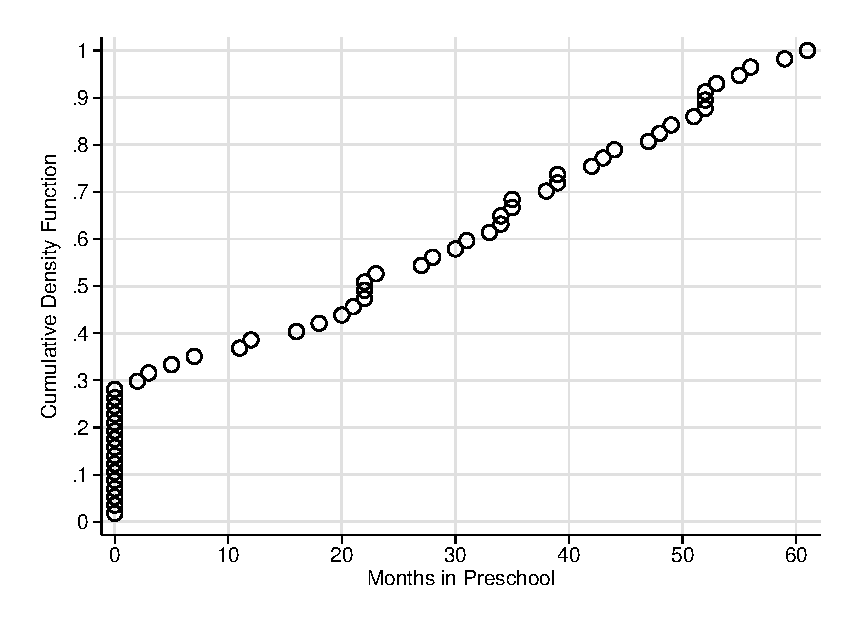
\includegraphics[width=.9\columnwidth]{output/abc_controlcontamination_months.eps}
\floatfoot{
\footnotesize
\noindent Note: This figure displays the cumulative density function of enrollment in alternative preschools of the control group in ABC.}
\end{figure}


%References
\singlespace
\bibliographystyle{chicago}
\bibliography{heckman}

\end{document} 